\section{社群识别与聚类}

\subsection{数据探索}

在进行社群识别之前,我们首先对数据进行一个粗略的分析。我们统计了每个子学科的节点数、任一端点位于学科内的边的数量、边的两个端点均属于该学科的边的数量及比例以及学科节点占总节点的比例。统计结果如表\ref{tab:Ratio}所示。

\begin{table}[h!]
\centering
\caption{Mathlib4中子学科的统计数据}
\begin{tabular}{llllll}
    \toprule
    Subject & Nodes & Edges & EdgesInSameSubject & EdgesRatio & NodesRatio\\ 
    \midrule
    Algebra & 894 & 6058 & 1939 & 0.32 & 0.18\\
    AlgebraicGeometry & 70 & 303 & 100 & 0.33 & 0.01\\
    AlgebraicTopology & 43 & 171 & 53 & 0.31 & 0.01\\
    Analysis & 488 & 2708 & 972 & 0.36 & 0.10\\
    CategoryTheory & 591 & 3351 & 1403 & 0.42 & 0.12\\
    Combinatorics & 107 & 429 & 112 & 0.26 & 0.02\\
    Computability & 18 & 66 & 15 & 0.23 & 0.00\\
    Condensed & 25 & 121 & 33 & 0.27 & 0.01\\
    Control & 25 & 112 & 28 & 0.25 & 0.01\\
    Data & 576 & 3144 & 801 & 0.25 & 0.12\\
    Dynamics & 23 & 95 & 16 & 0.17 & 0.00\\
    FieldTheory & 52 & 292 & 71 & 0.24 & 0.01\\
    Geometry & 80 & 311 & 109 & 0.35 & 0.02\\
    GroupTheory & 119 & 649 & 157 & 0.24 & 0.02\\
    InformationTheory & 1 & 1 & 0 & 0.00 & 0.00\\
    LinearAlgebra & 233 & 1411 & 402 & 0.28 & 0.05\\
    Logic & 50 & 383 & 55 & 0.14 & 0.01\\
    MeasureTheory & 196 & 1001 & 350 & 0.35 & 0.04\\
    ModelTheory & 29 & 118 & 41 & 0.35 & 0.01\\
    NumberTheory & 149 & 643 & 168 & 0.26 & 0.03\\
    Order & 209 & 1281 & 331 & 0.26 & 0.04\\
    Probability & 61 & 221 & 85 & 0.38 & 0.01\\
    RepresentationTheory & 15 & 83 & 18 & 0.22 & 0.00\\
    RingTheory & 368 & 2169 & 638 & 0.29 & 0.07\\
    SetTheory & 46 & 216 & 55 & 0.25 & 0.01\\
    Topology& 442 & 2379 & 820 & 0.34 & 0.09\\
    \bottomrule
\end{tabular}
\label{tab:Ratio}
\end{table}

我们知道,对于一张随机图,当NodesRatio较小时,EdgesRatio应大致为NodesRatio的一半,而实际上EdgesRatio远大于NodesRatio的一半,说明这张图中确实存在社群结构,且该结构一定程度上被学科分类所反映。可以算出,按学科进行分类的modularity为0.527, 说明学科分类对于该图的社群结构有着一定的解释力。

\subsection{谱聚类}

我们下面尝试使用谱聚类的方法来找到这些社群。
我们使用\texttt{sklearn.cluster}中的\texttt{Spectral-\allowbreak Clustering}来进行谱聚类,我们将谱聚类的结果与学科分类进行比较,以此来验证该图中的社群是否与按学科划分的社群一致;当然谱聚类本身对社群的划分效果也要做衡量,为此选用Adjusted Rand Index (ARI)、Normalized Mutual Information (NMI)和modularity来作为聚类效果的评价指标。考虑到我们一共有26个子学科,虽然不是每一个学科都很好的形成一个极大的社群,但是大致地将聚类数选成26是合理的。后续我们遍历了2到30的聚类数,最优的聚类数大致在二十多,但实际上,聚类效果的好坏对随机因素相当敏感,选取26作为聚类数的效果并不显著优于或劣于选取21到26之间的其他聚类数。我们对谱聚类的结果进行了可视化,如图\ref{fig:clustering}所示。对应的评价指标如表\ref{tab:score}所示。
\begin{figure}[htb]
    \centering
    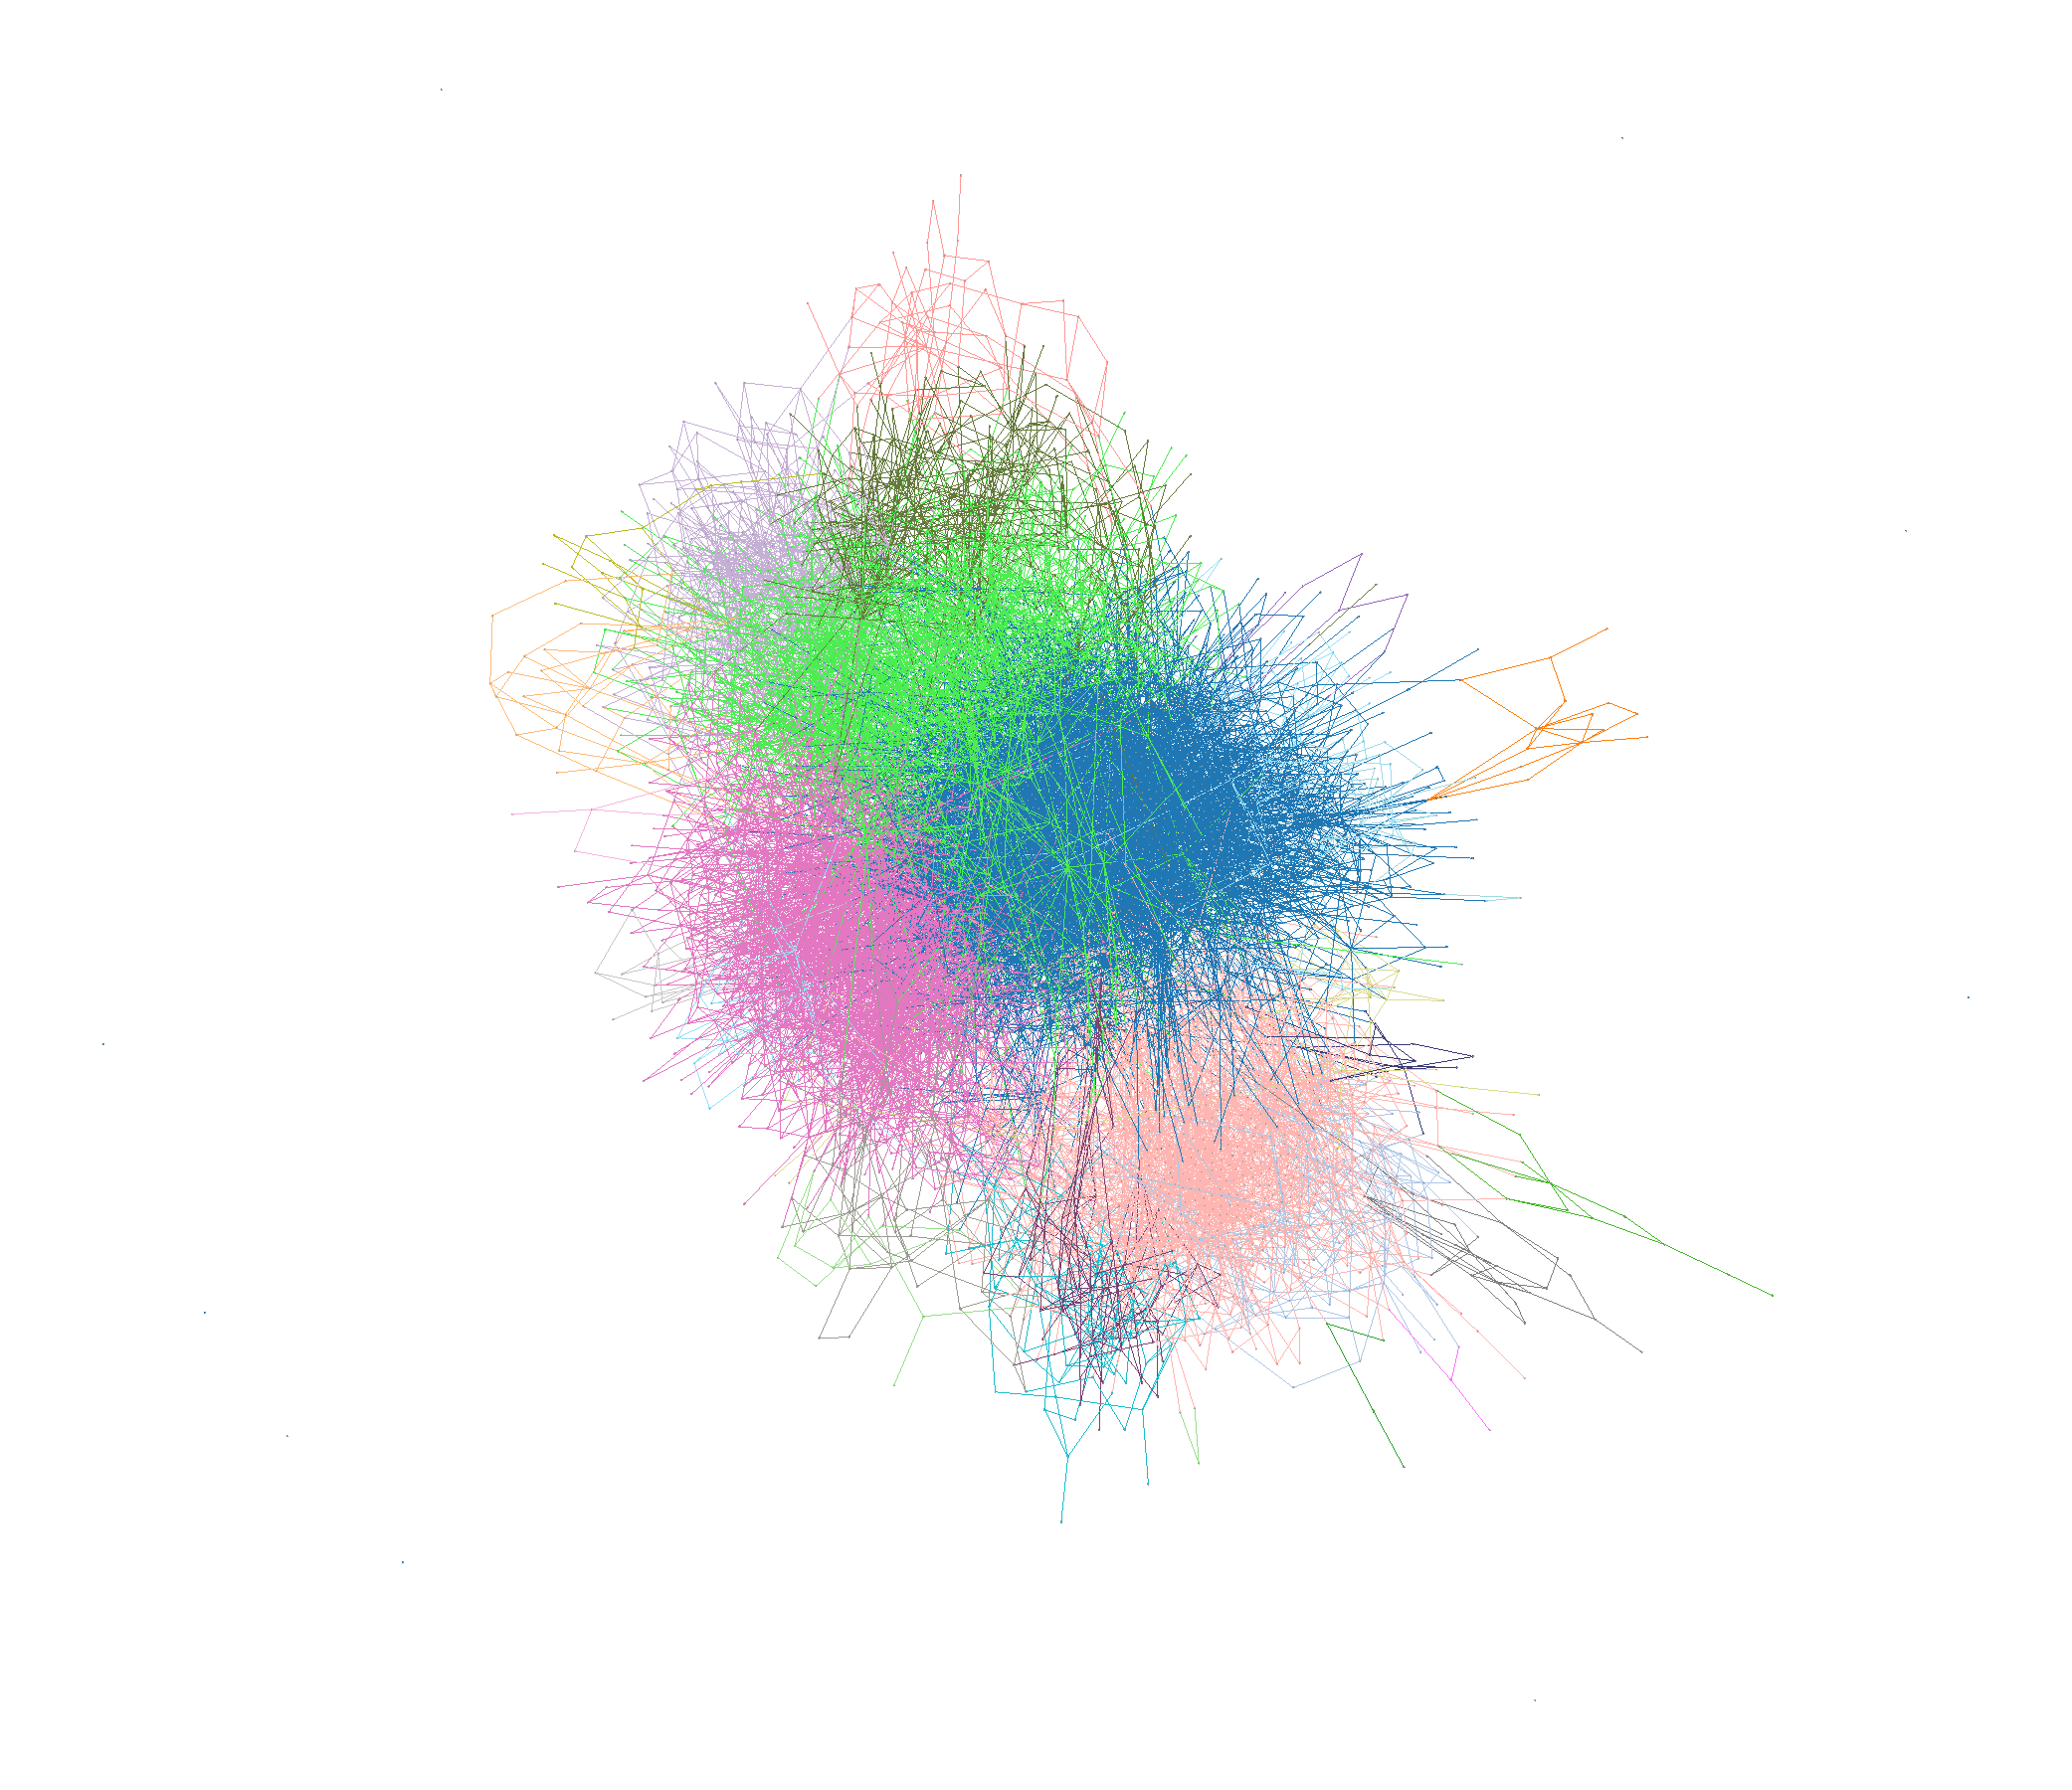
\includegraphics[width=.7\textwidth]{../solve/img/graph_spectral_cluster.png}
    \caption{谱聚类后的Mathlib4依赖关系图}
    \label{fig:clustering}
\end{figure}
\begin{table}[htb]
  \centering
  \caption{Evaluation scores of spectral clustering}
  \begin{tabular}{lll}
    \toprule
    ARI & NMI & Modularity\\
    \midrule
    0.260 & 0.475 & 0.614\\
    \bottomrule
  \end{tabular}
  \label{tab:score}
\end{table}

较高的modularity表明聚类效果良好,Mathlib4中的数学概念之间确实有着非常明确的社群结构且该结构被谱聚类很好地捕捉了,但较为一般的ARI和NMI表明谱聚类的结果与学科分类并不完全一致,这是因为Mathlib4中的数学概念之间的依赖关系并不完全由学科决定,而是由数学概念之间的逻辑关系决定的,实际上考虑到使用谱聚类的modularity比按学科分类的modularity要高出9个百分点,我们认为谱聚类的结果与按学科分类的结果不完全一致是符合预期的。

\subsection{SBM模型}
接下来我们使用\texttt{graph\_tool}库中的SBM模型来对Mathlib4进行社群识别。我们分别使用\texttt{graph\_tool}的\texttt{minimize\_blockmodel\_dl}函数和\texttt{minimize\_nested\_blockmodel\_dl}函数来对Mathlib4进行社群识别,得到的结果如图\ref{fig:SBM_combined}所示。

\begin{figure}[htb]
  \centering
  \begin{subfigure}[b]{0.45\textwidth}
    \centering
    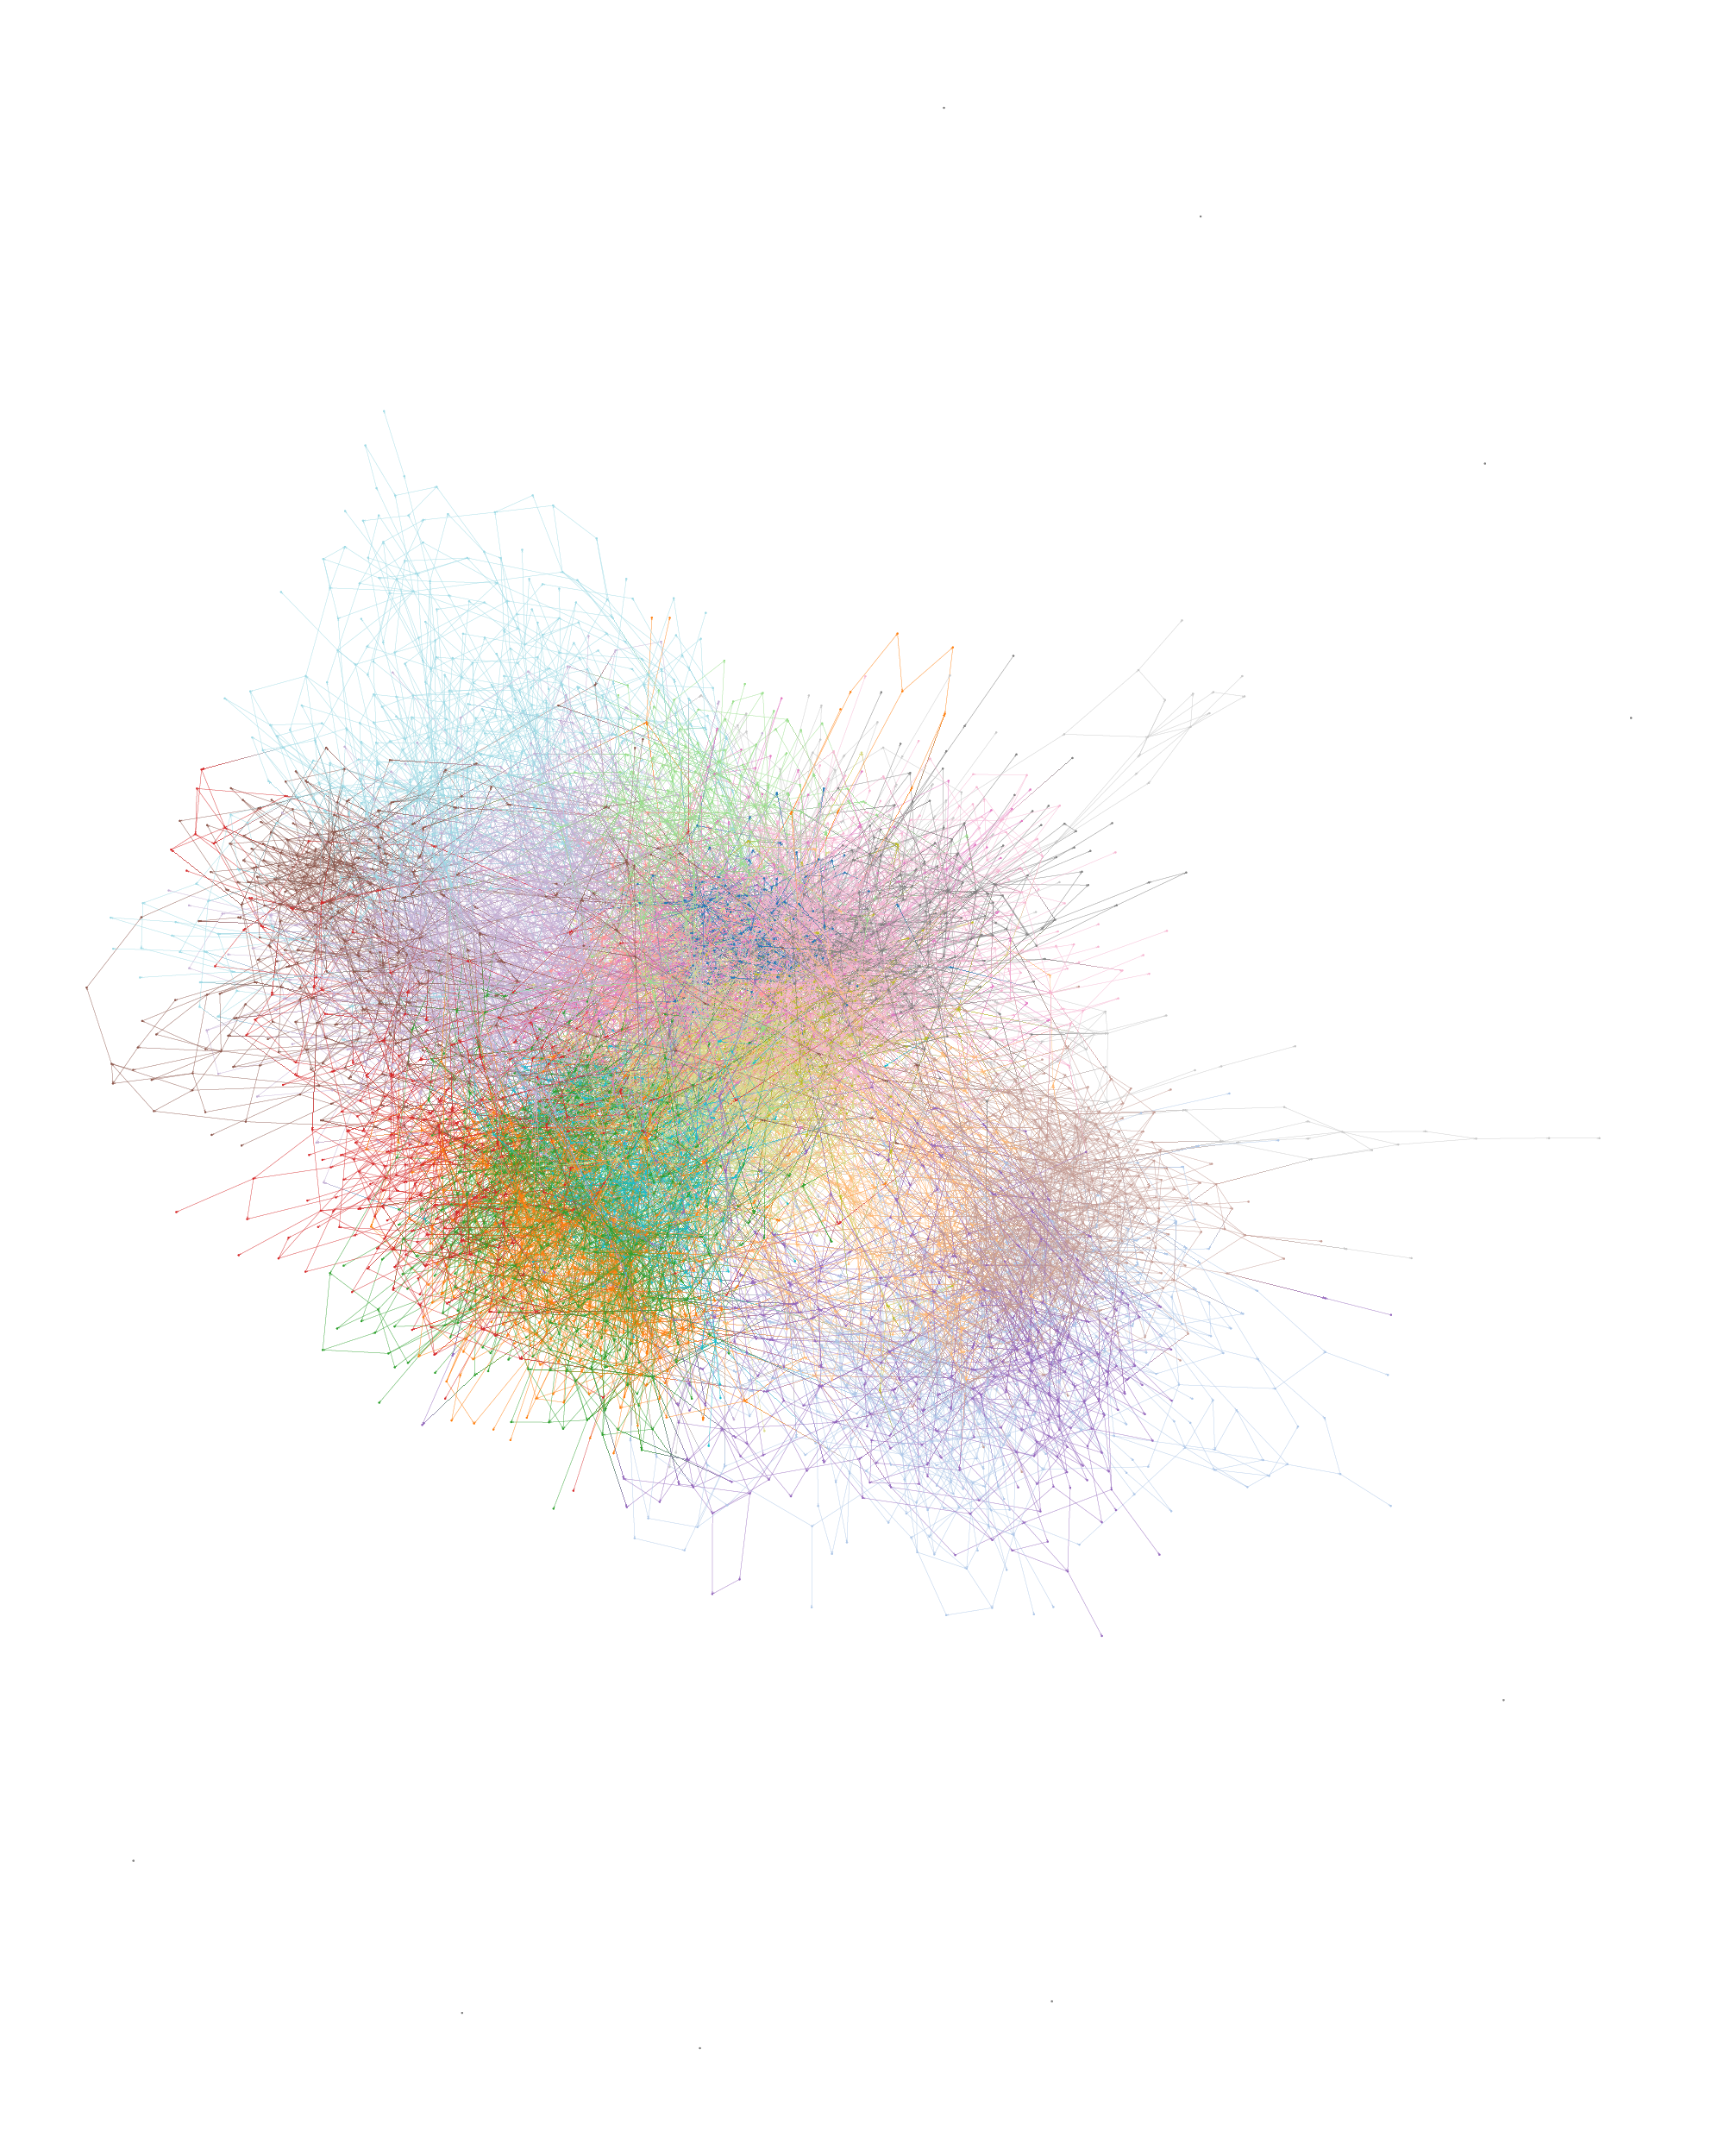
\includegraphics[width=\textwidth, trim=0cm 10cm 0cm 10cm, clip]{../solve/img/SBM.png}
    \caption{SBM模型}
    \label{fig:SBM}
  \end{subfigure}
  \hfill
  \begin{subfigure}[b]{0.45\textwidth}
    \centering
    \includegraphics[width=\textwidth]{../solve/img/SBM_nested.png}
    \caption{嵌套SBM模型}
    \label{fig:nest_SBM}
  \end{subfigure}
  \caption{按SBM模型着色的Mathlib4依赖关系图}
  \label{fig:SBM_combined}
\end{figure}

对应的评价指标如表\ref{tab:score2}所示。
\begin{table}[h!]
  \centering
  \caption{SBM模型的评价指标}
  \begin{tabular}{llll}
    \toprule
    Model & ARI & NMI & Modularity\\
    \midrule
    SBM & 0.226 & 0.466 & 0.614\\
    nested SBM & 0.199 & 0.450 & 0.614\\
    \bottomrule
  \end{tabular}
  \label{tab:score2}
\end{table}

可以看到,SBM模型的modularity与谱聚类的modularity相同,而ARI和NMI稍低,这说明SBM模型的结果与谱聚类的结果基本一致。

总的来说,谱聚类和SBM模型都能够很好地识别出Mathlib4中的社群结构,但是谱聚类和SBM模型的结果与学科分类的结果有一定的差异,而SBM模型的结果与谱聚类的结果基本一致。这说明Mathlib4中存在社群结构,学科分类一定程度上可以解释这个社群结构,但是社群结构并不完全由学科分类决定。





